%\chapter*{Неделя 9}
\protect\thispagestyle{fancy}
\section{}
На рисунке приведена блок-схема системы однократной передискретизации с рациональным шагом $L/M$.

\begin{figure}[!h]
	\centering
	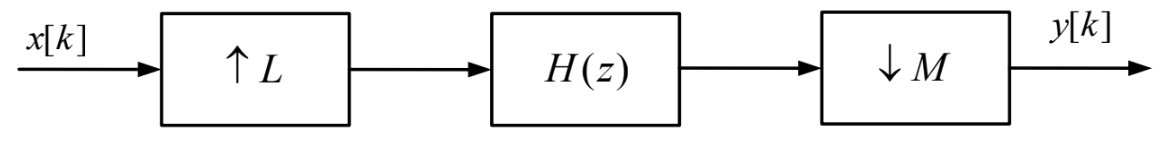
\includegraphics[width=1.\columnwidth]{pics/spring/8/810.png}
	%\caption{.}
	\label{fig:8-1-0}
\end{figure}

Постройте график для АЧХ идеального фильтра в данной системе однократной передискретизации для следующих случаев:

\begin{enumerate}[label=(\alph*)]
	\item $L=3$ и $M=2$;
	\item $L=2$ и $M=3$.
\end{enumerate}

\begin{equation*}
|\mathcal{H}_{id}(\tilde{\nu})| = \begin{cases}
L,\quad |\tilde{\nu}| \leq \min\left\{\dfrac{1}{2L}, \dfrac{1}{2M}\right\};\\
0,\quad \text {для других } \tilde{\nu} \in [-0.5, +0.5].
\end{cases}
\end{equation*}

\begin{figure}[!h]
	\centering
	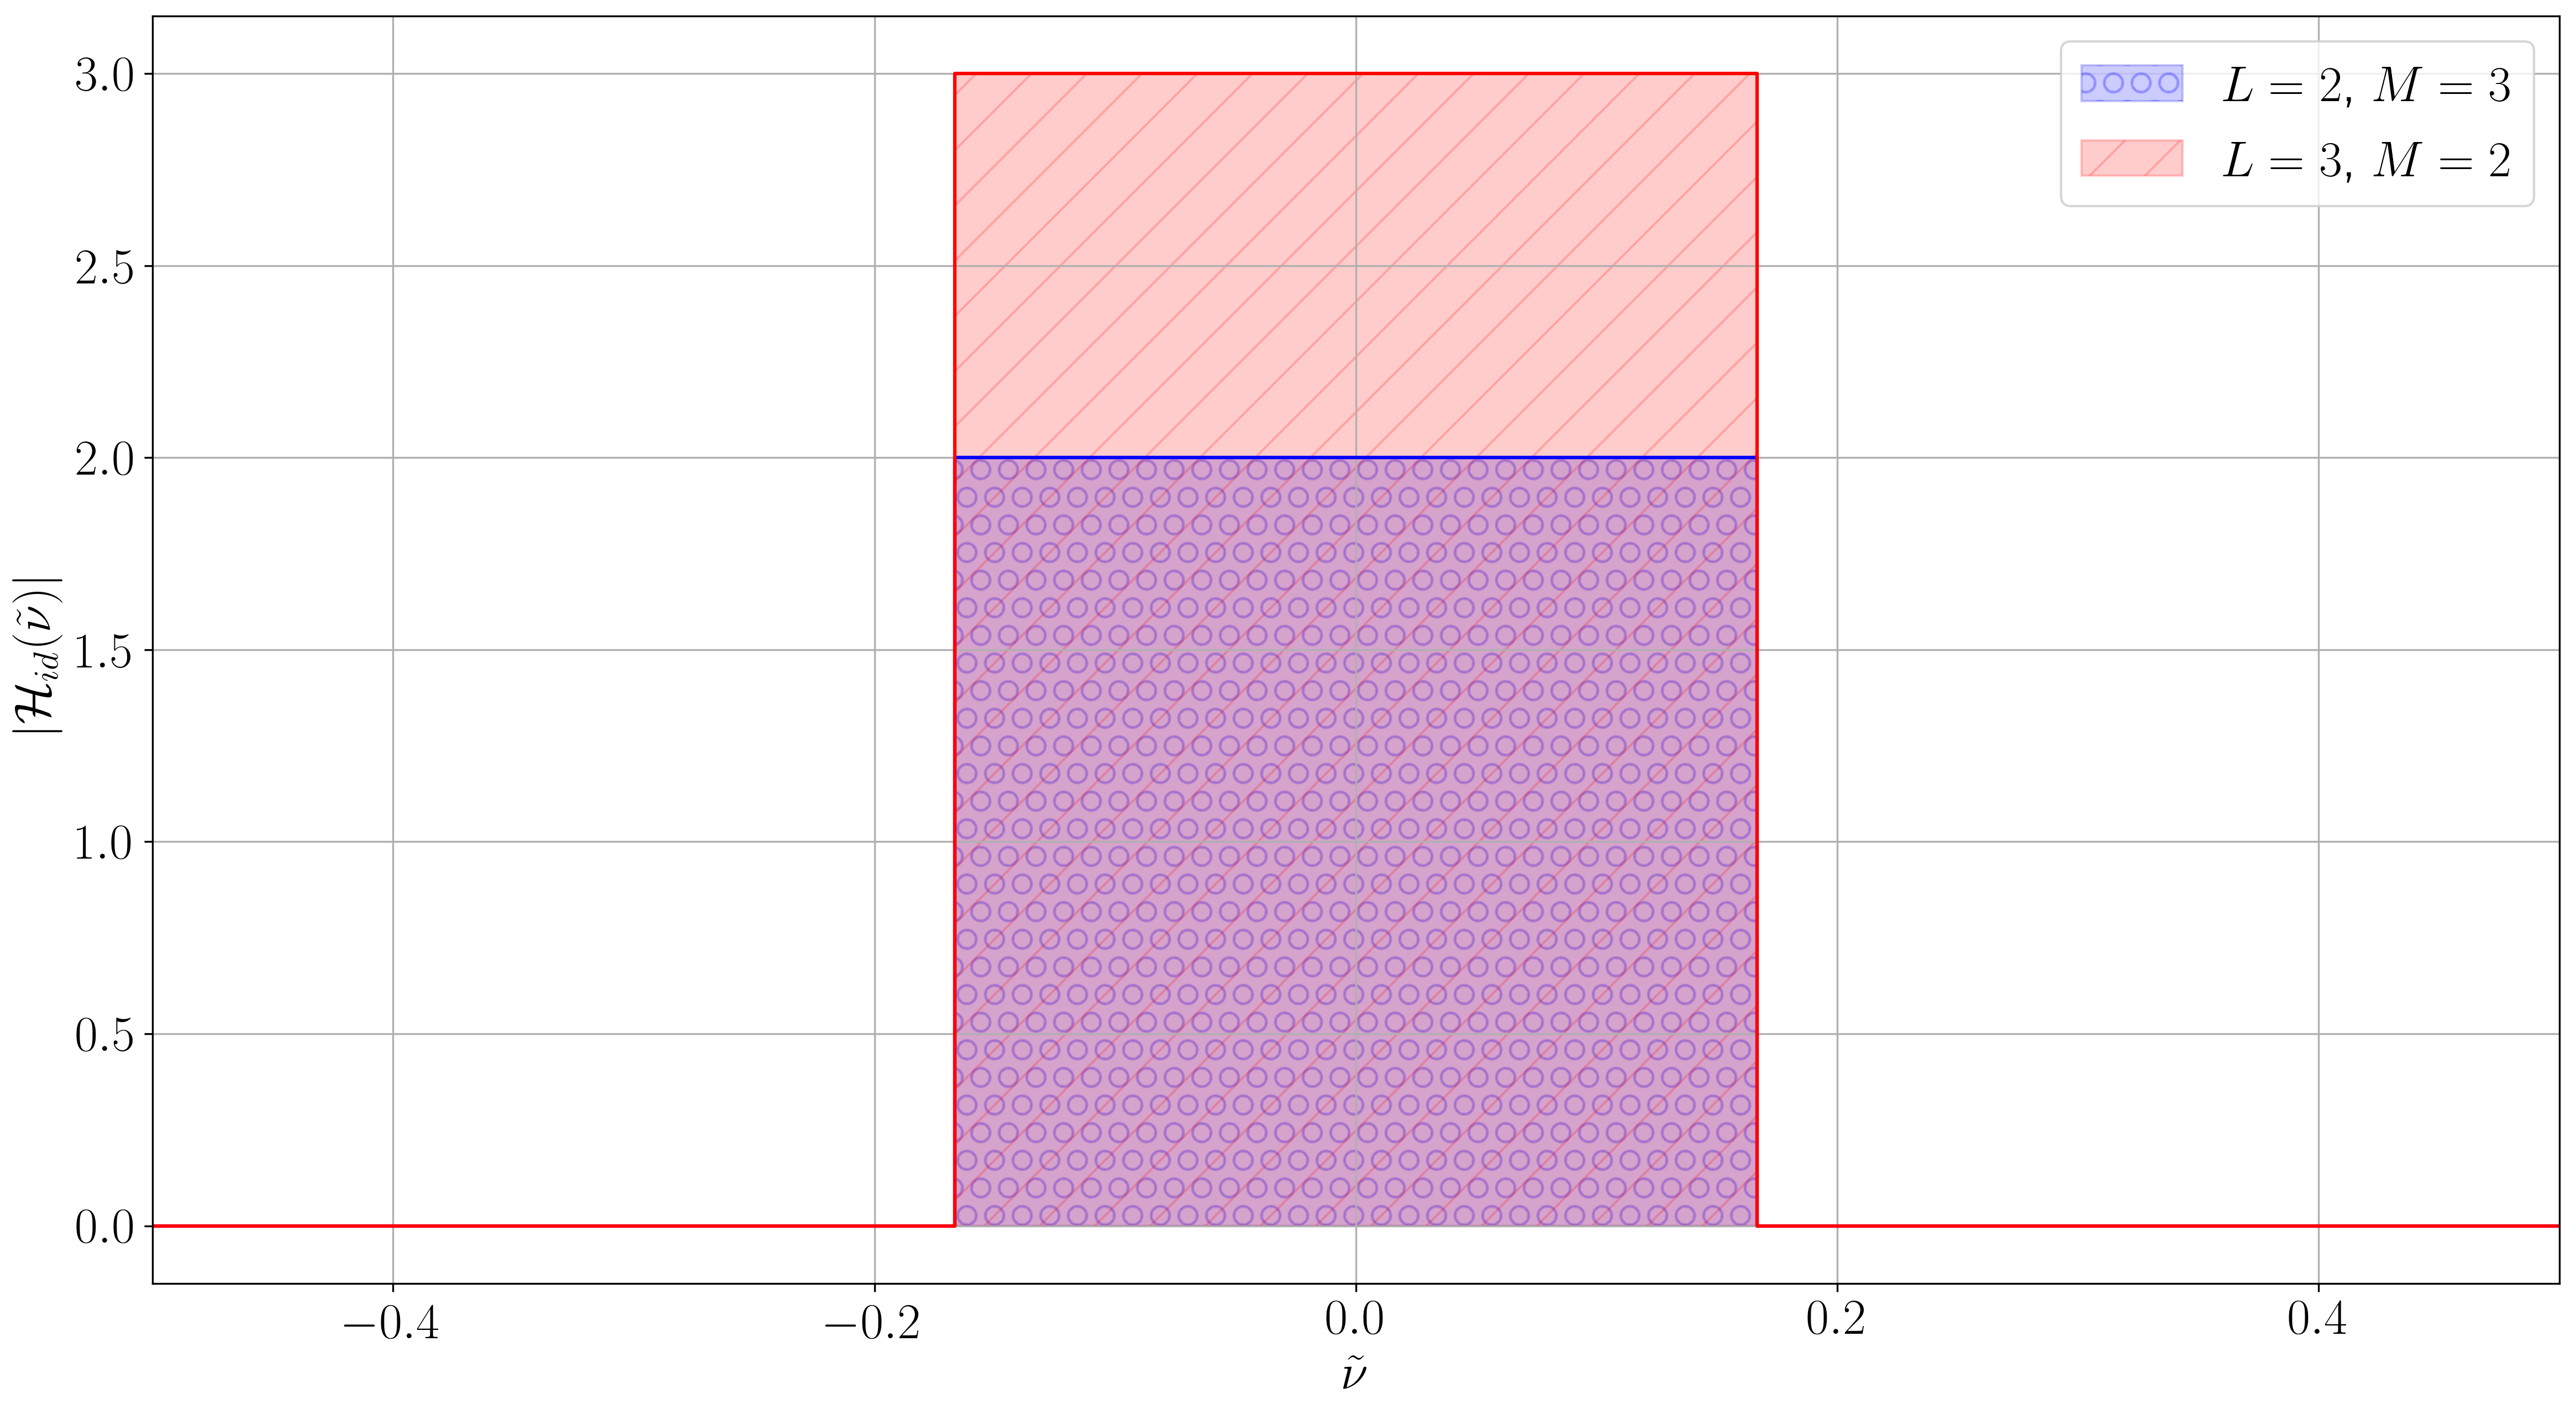
\includegraphics[width=0.9\columnwidth]{pics/spring/8/8-1.png}
	%\caption{.}
	\label{fig:8-1}
\end{figure}

\newpage
\section{}
На рисунке приведена блок-схема системы однократной интерполяции с целыми коэффициентом $L$.

\begin{figure}[!h]
	\centering
	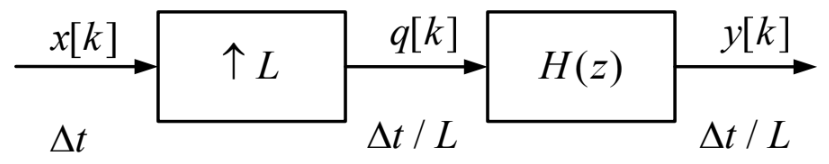
\includegraphics[width=0.8\columnwidth]{pics/spring/8/820.png}
	%\caption{.}
	\label{fig:8-2-0}
\end{figure}

Предположим, что гармонический сигнал $x(t) = \cos (2\pi f_0 t)$ дискретизуется так, что на периоде $[0; 1/f_0)$ образуется $8$ отсчётов $\tilde{x}[k] = x(k\Delta t)$, $f_d=1/\Delta t$.
Далее последовательность $x[k]$ длиной в $16$ отсчётов поступает на вход системы однократной интерполяции с коэффициентом $L=2$.
\begin{equation*}
x[k] = \begin{cases}
\tilde{x}[k], \text{ при } 0 \leq k < 16;\\
0, \text{ при других } k,
\end{cases}
\end{equation*}

Построить графики
\begin{enumerate}[label=(\alph*)]
	\item последовательностей $x[k]$ и $q[k]$;
	\item модуля ДВПФ последовательностей $x[k]$ и $q[k]$
	в нормированных	частотах $\nu = f/f_d$;
	\item модуля ДВПФ последовательности $y[k]$	в нормированных частотах $\nu = f/f_d$ при условии, что $q[k]$ поступает на вход идеального фильтра	нижних частот системы однократной интерполяции;
	\item графики модуля ДВПФ $x[k]$ и $y[k]$ для частот $f \in [-0.5f_d; +2.5f_d]$ (в Гц).
\end{enumerate}

\begin{figure}[!h]
	\centering
	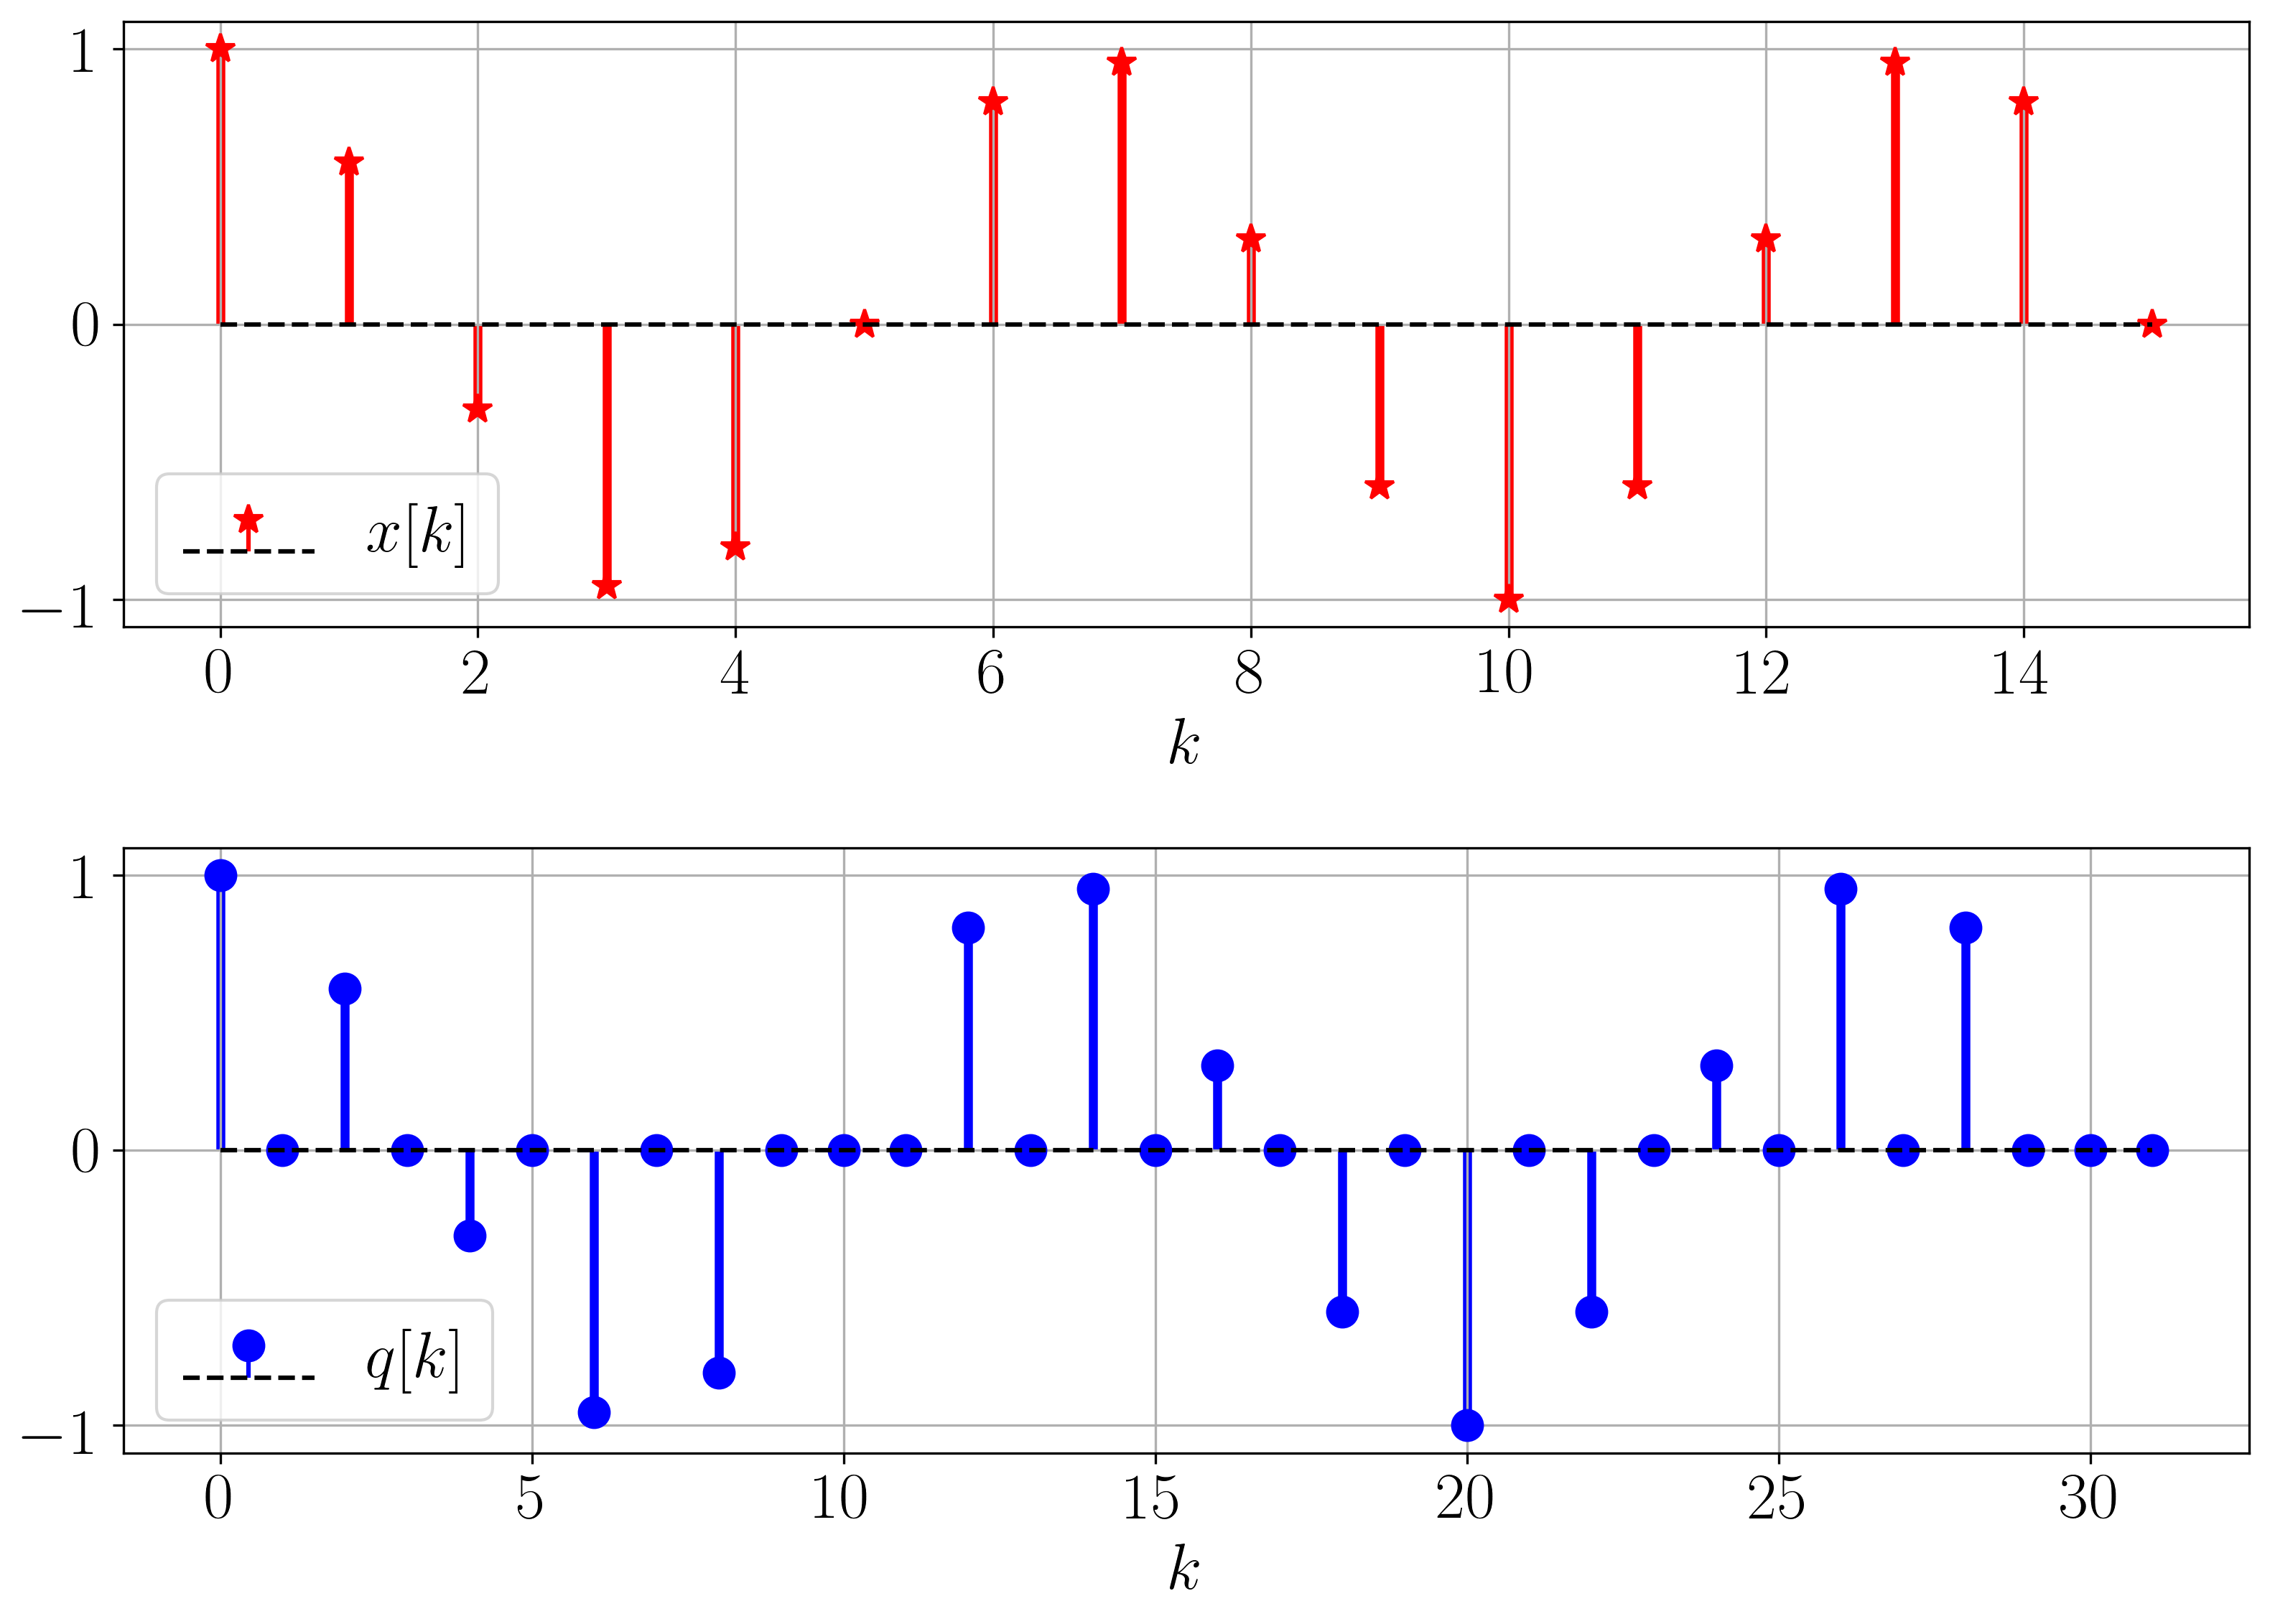
\includegraphics[width=0.7\columnwidth]{pics/spring/8/8-2-1.png}
	\label{fig:8-2-1}
\end{figure}

\begin{figure}[!h]
	\centering
	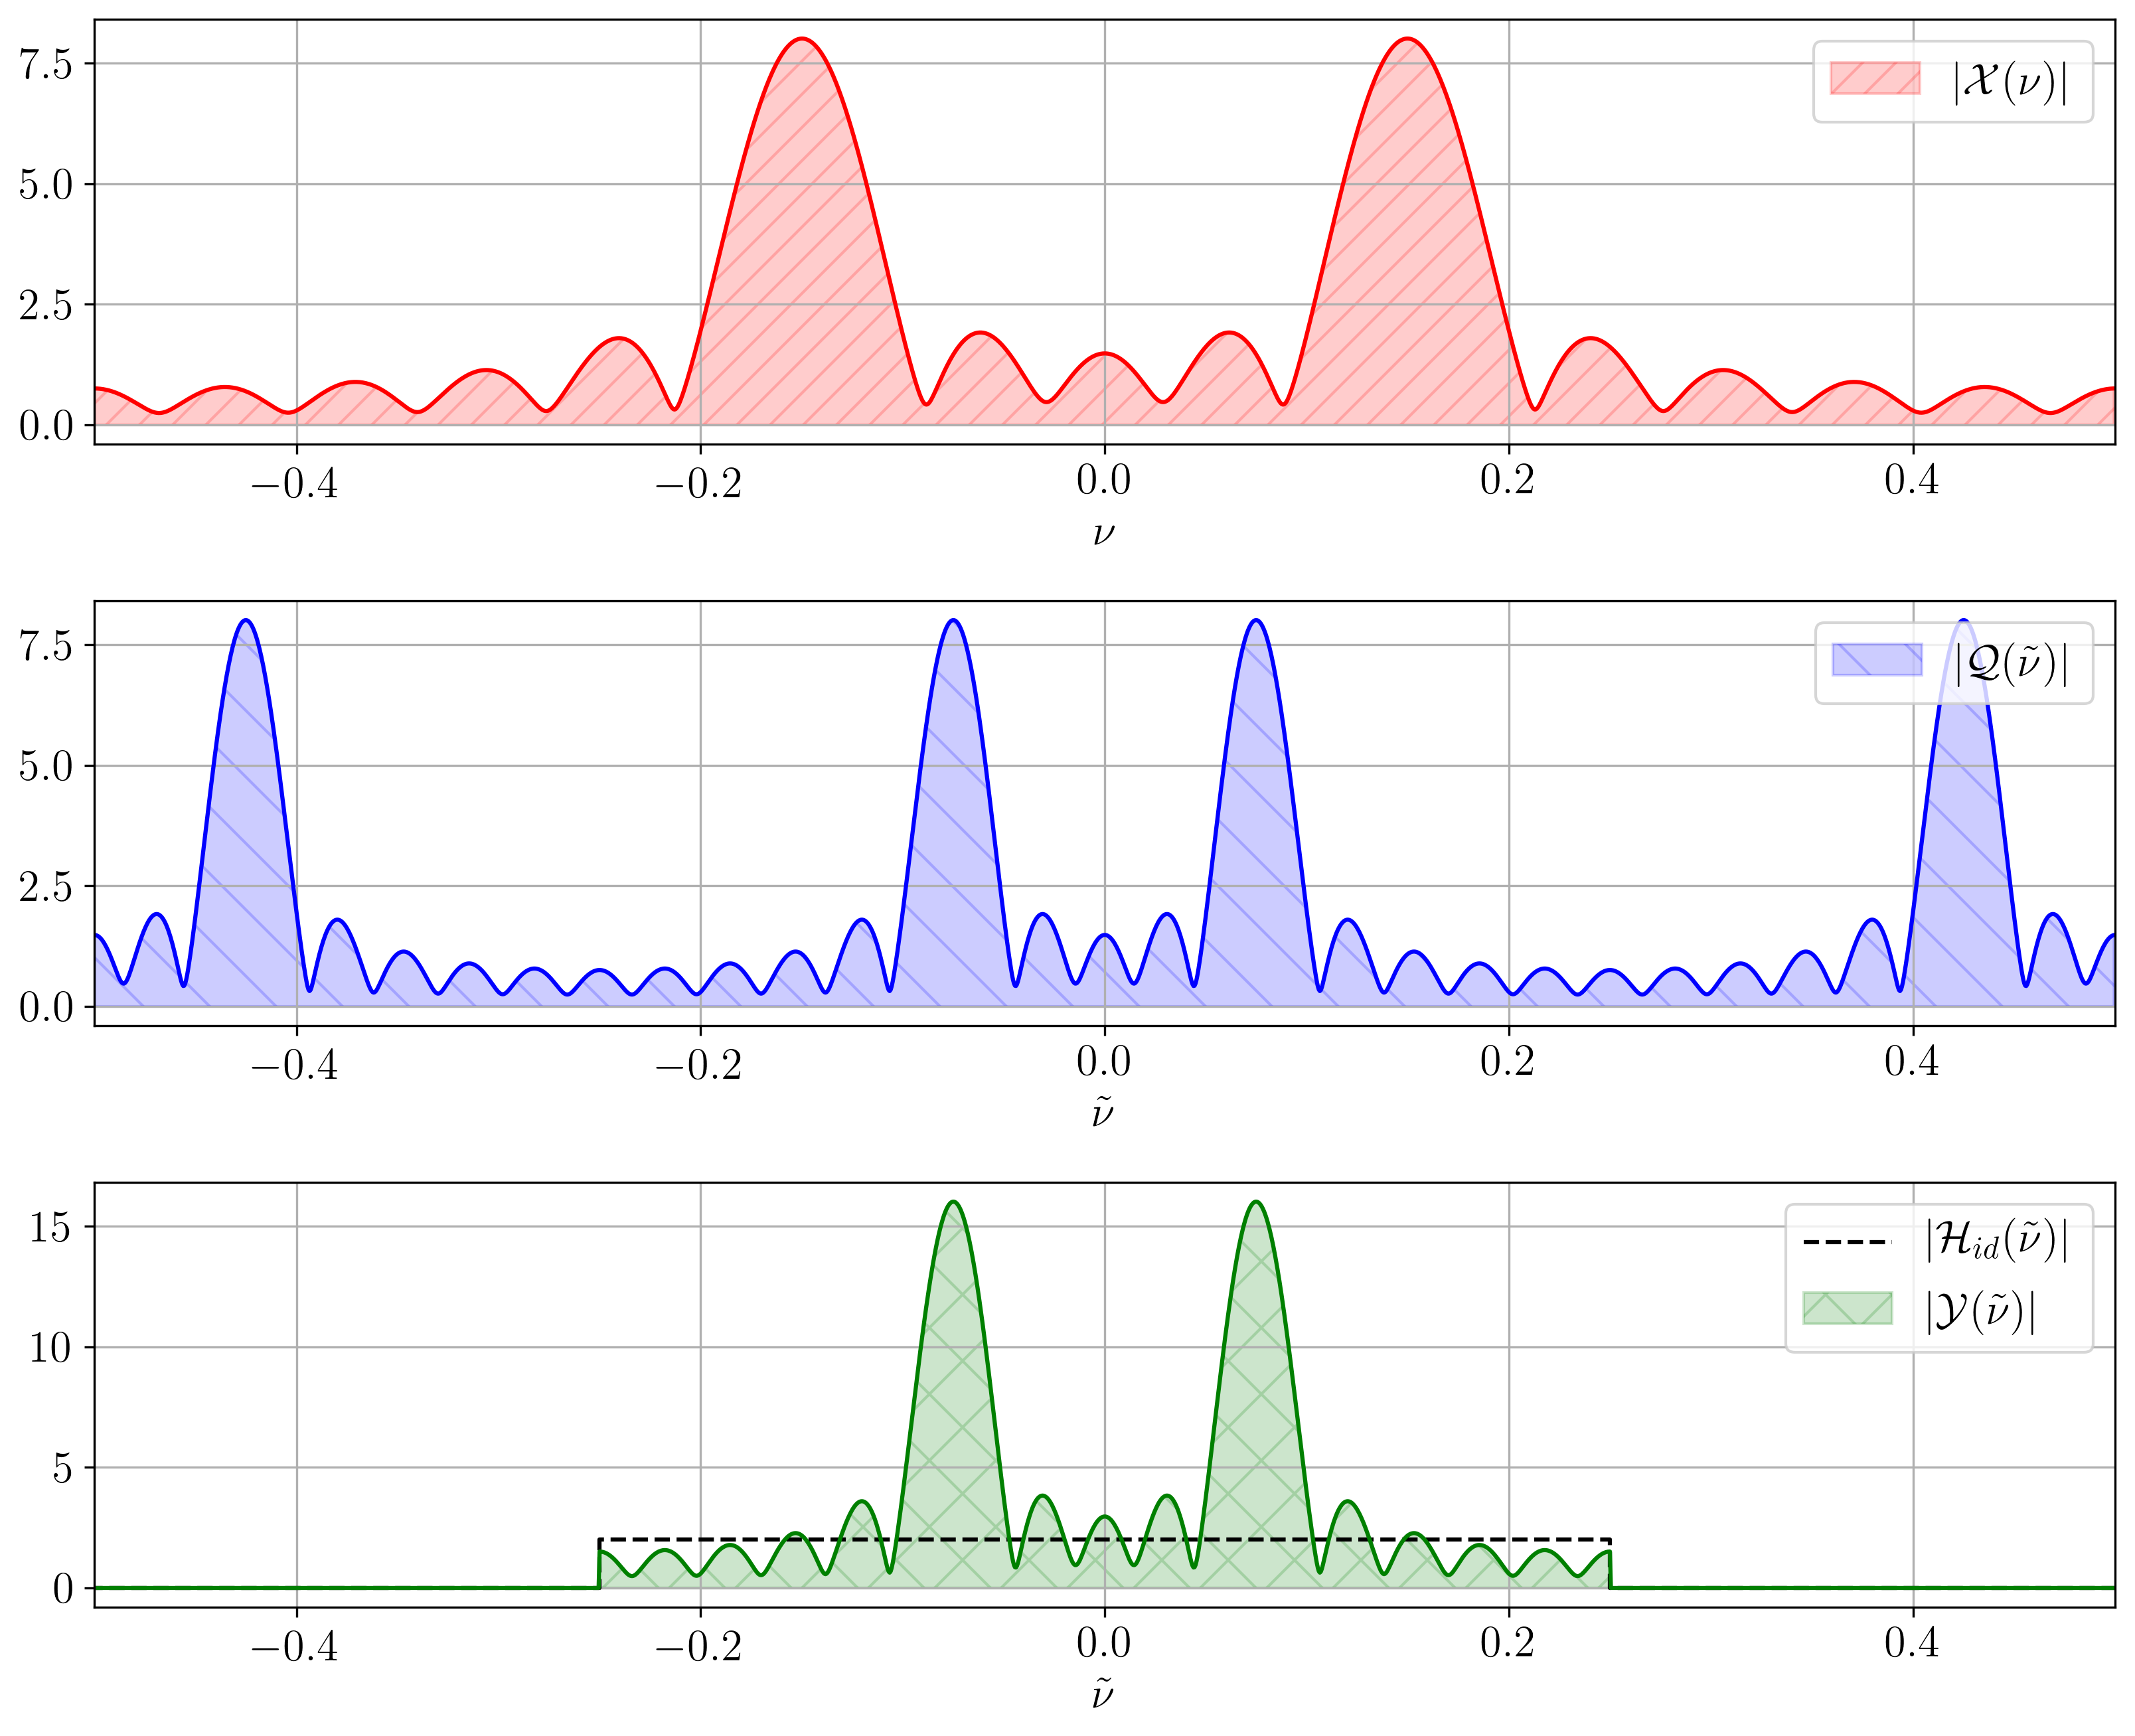
\includegraphics[width=0.85\columnwidth]{pics/spring/8/8-2-2.png}
	\label{fig:8-2-2}
\end{figure}

\begin{figure}[!h]
	\centering
	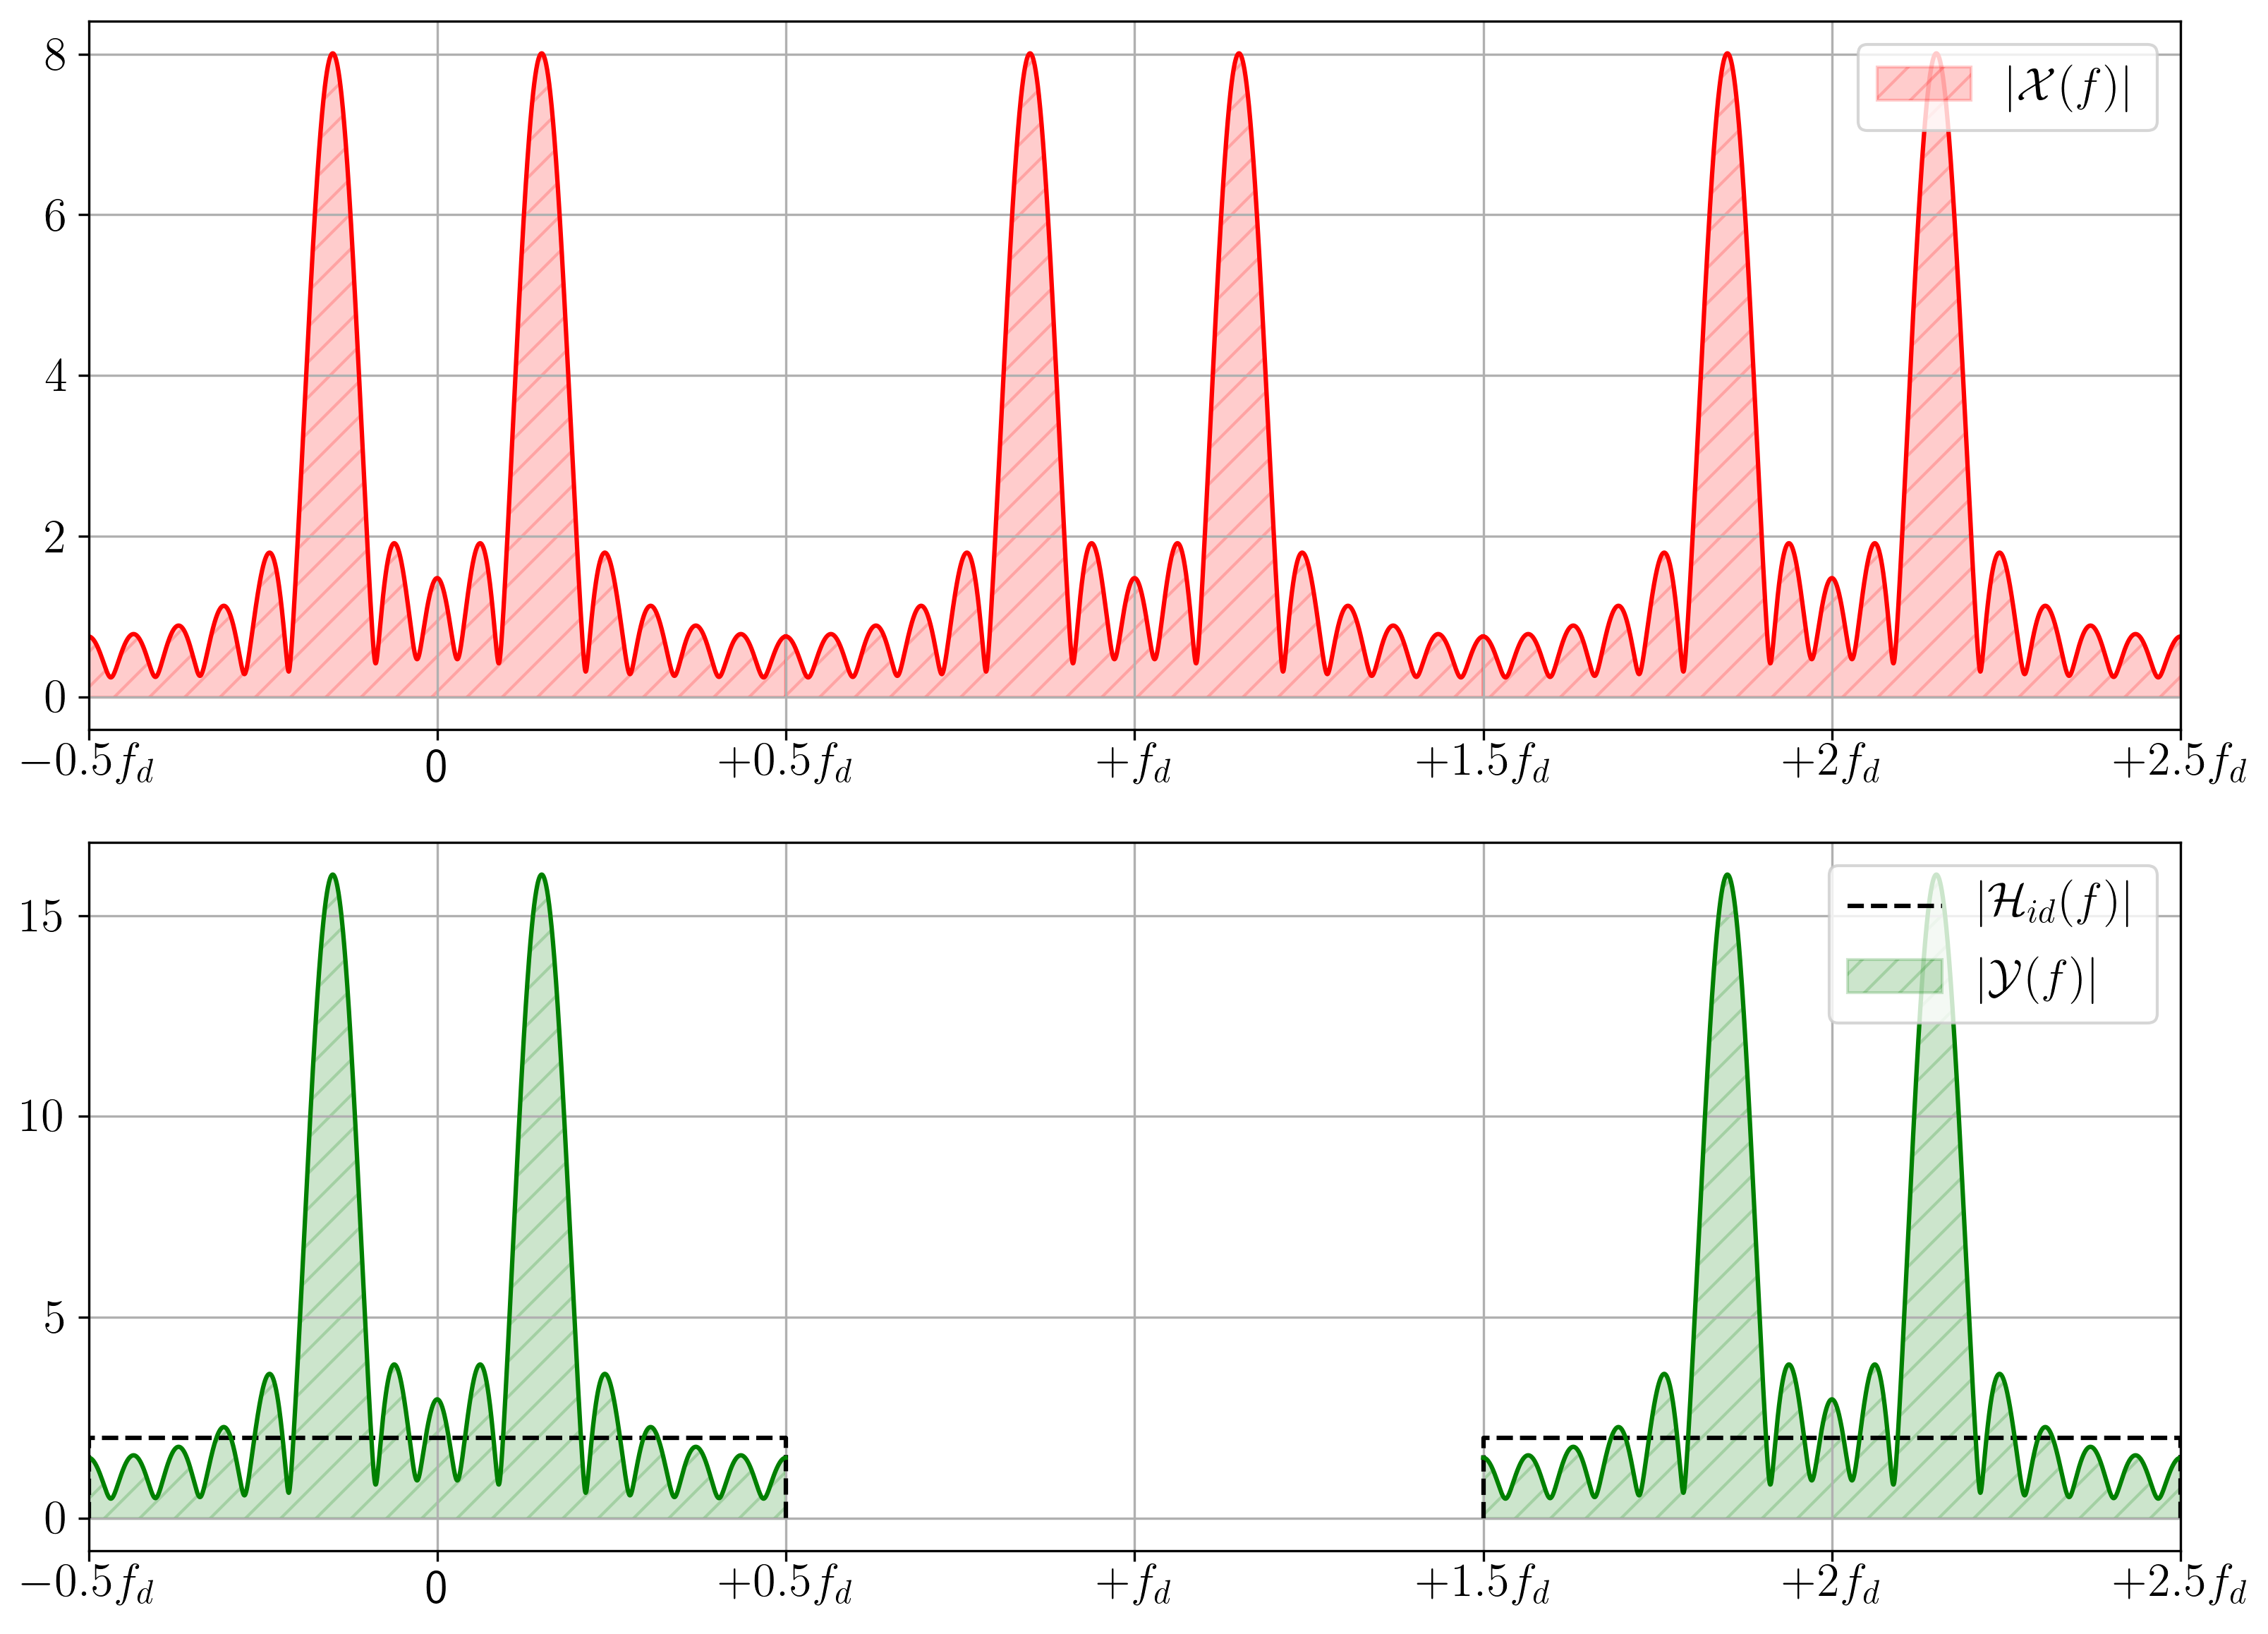
\includegraphics[width=0.85\columnwidth]{pics/spring/8/8-2-3.png}
	\label{fig:8-2-3}
\end{figure}

\newpage
\section{}
Предположим, что используется система однократной децимации с целым коэффициентом $M=2$ с идеальным ФНЧ.

\begin{figure}[!h]
	\centering
	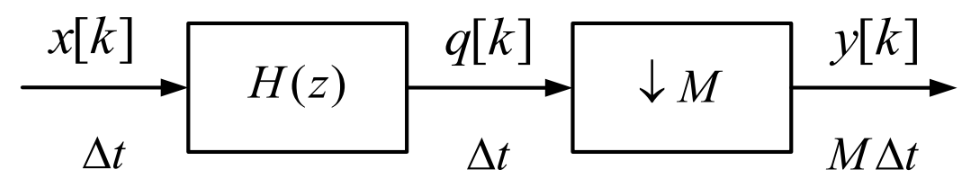
\includegraphics[width=0.8\columnwidth]{pics/spring/8/830.png}
	%\caption{.}
	\label{fig:8-3-0}
\end{figure}


Модуль ДВПФ входной последовательности $x[k]$ изображен на рисунке ниже, ее частота дискретизации $f_d$.

Построить для частот $f \in [-1.5f_d; +1.5f_d]$ (в Гц) графики модуля ДВПФ последовательностей
$q[k]$ (на выходе фильтра) и $y[k]$ (на выходе системы), а также АЧХ фильтра.

\begin{figure}[!h]
	\centering
	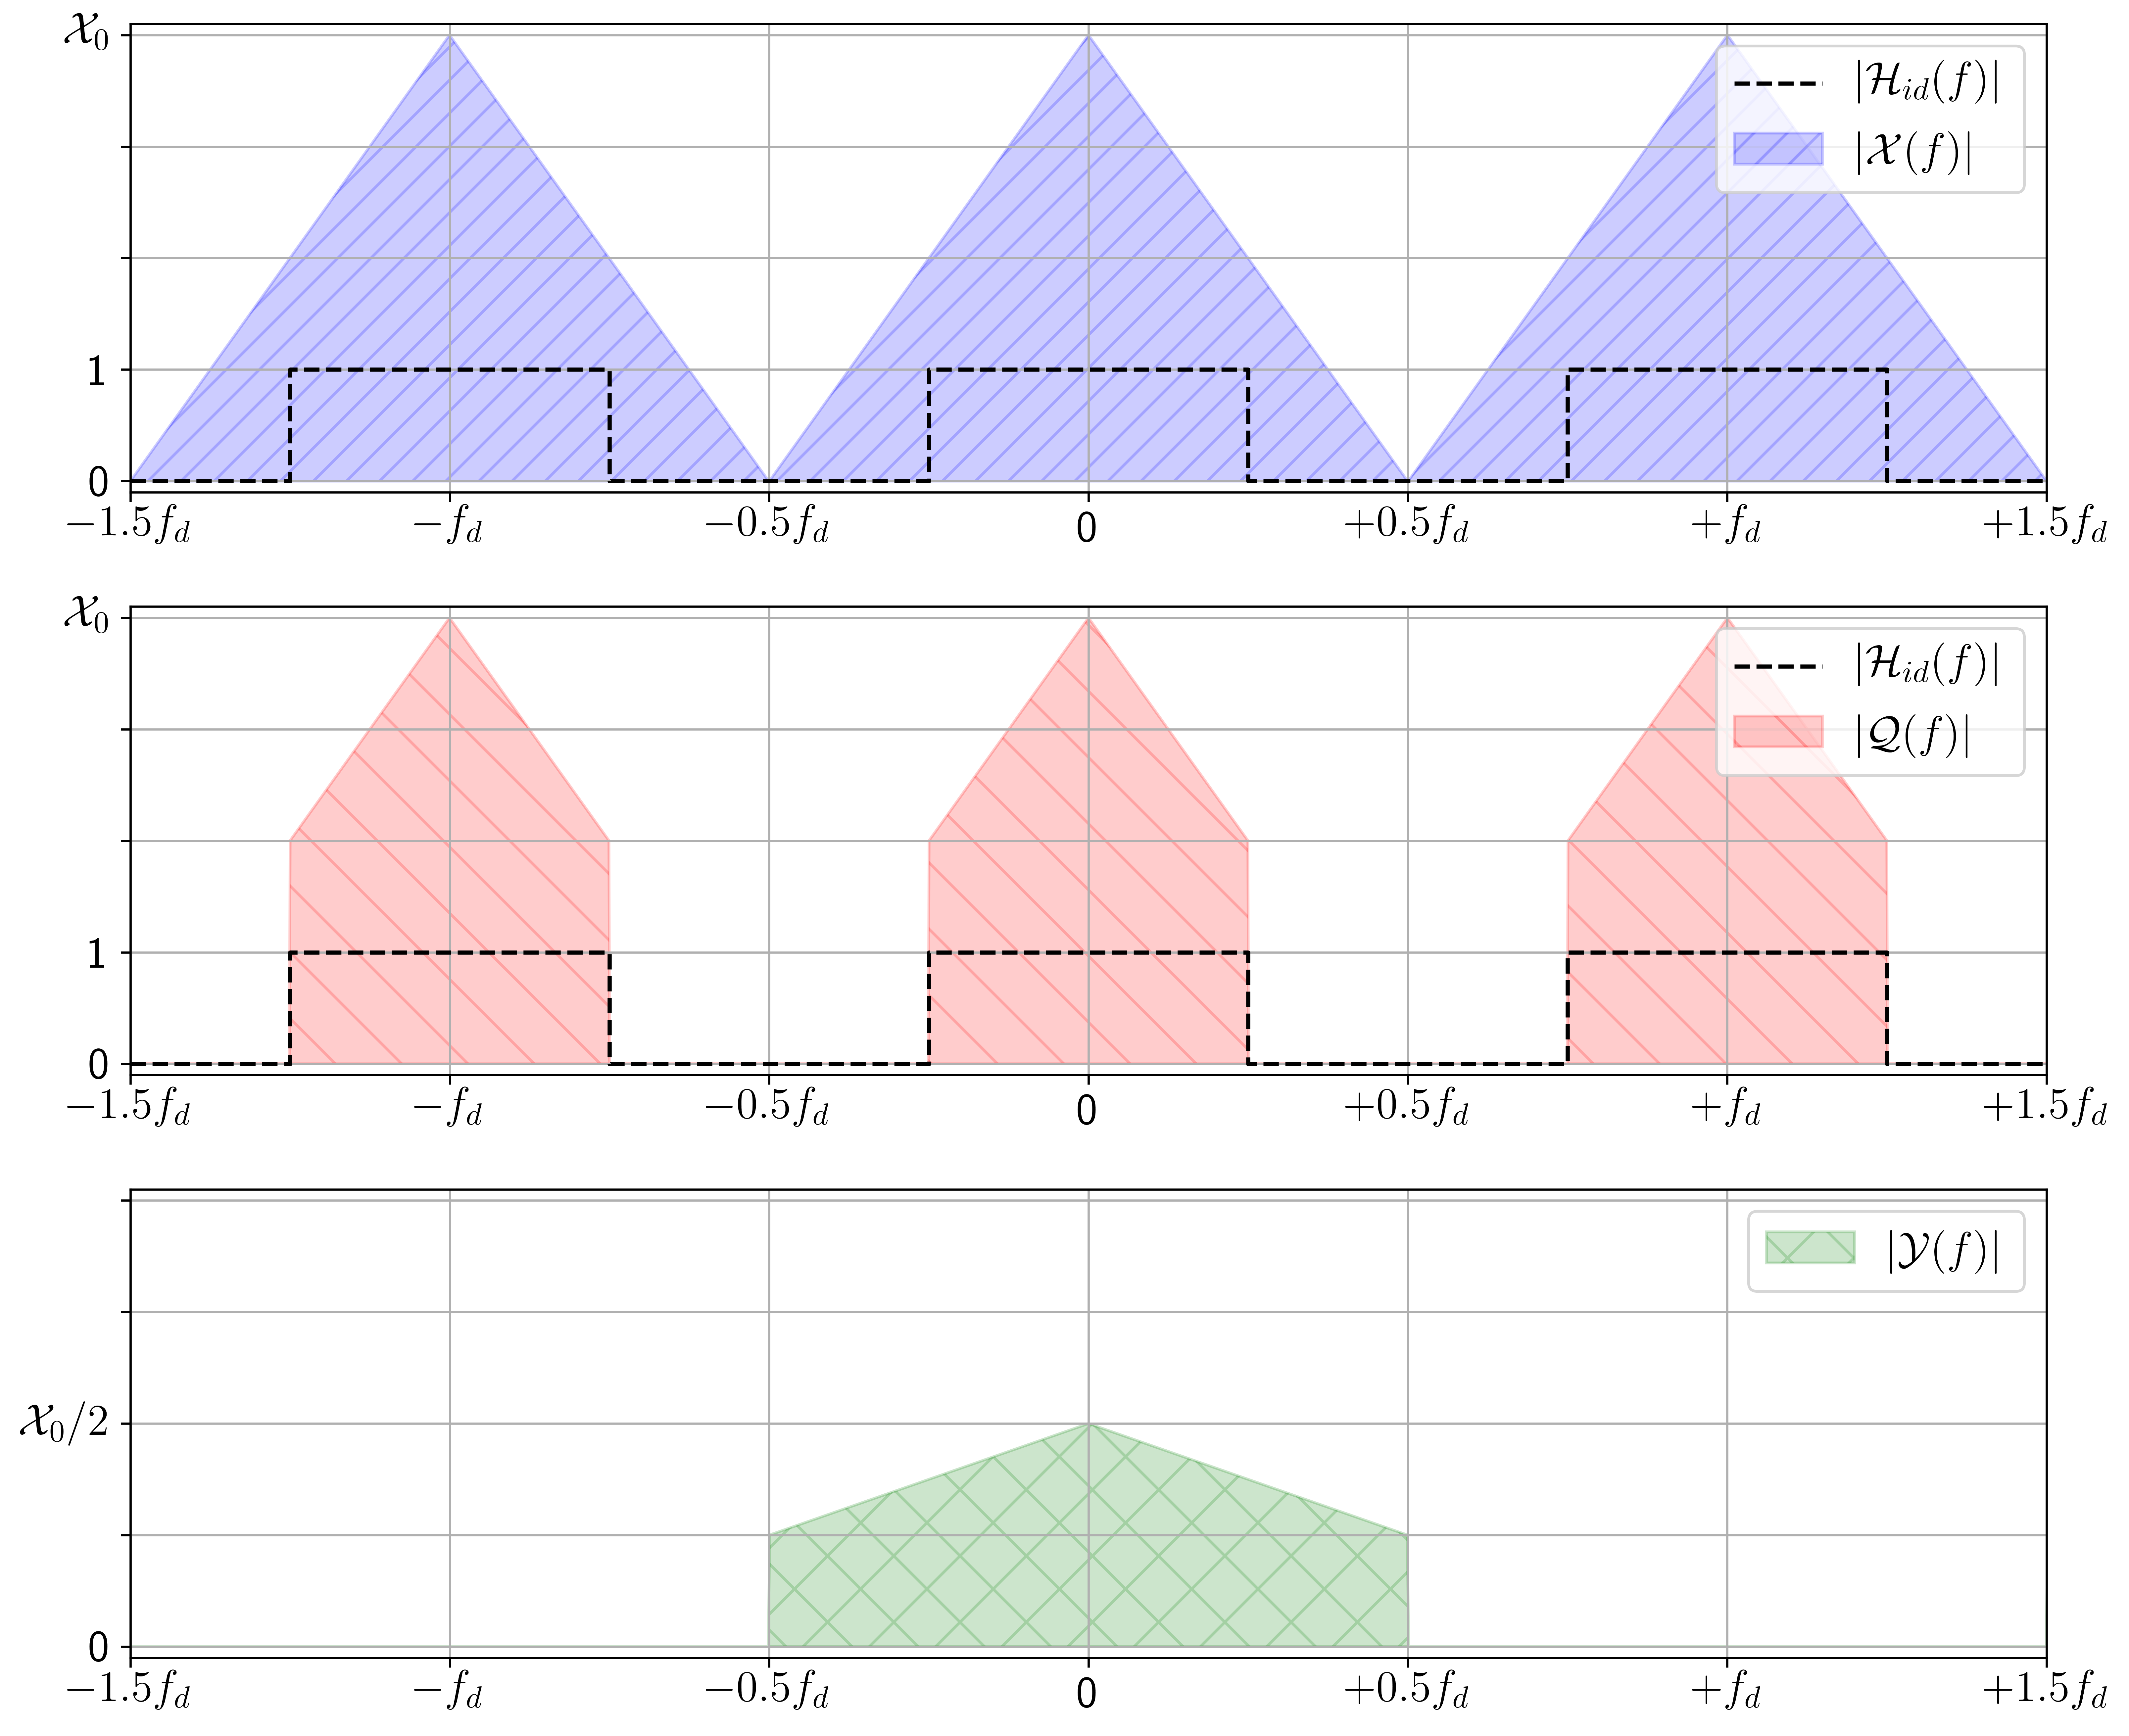
\includegraphics[width=1.0\columnwidth]{pics/spring/8/8-3.png}
	%\caption{.}
	\label{fig:8-3}
\end{figure}

